\documentclass[../main.tex]{subfiles}
\begin{document}

\section{Results}

The sequencing of these two genomes revealed they are highly similar in many aspects, and both assemble into circular-mapping molecules, containing 12 protein-coding genes, two rRNA genes, and four tRNA genes, see Figure 1 for detailed diagram.

\begin{figure}[htp]
    \centering
    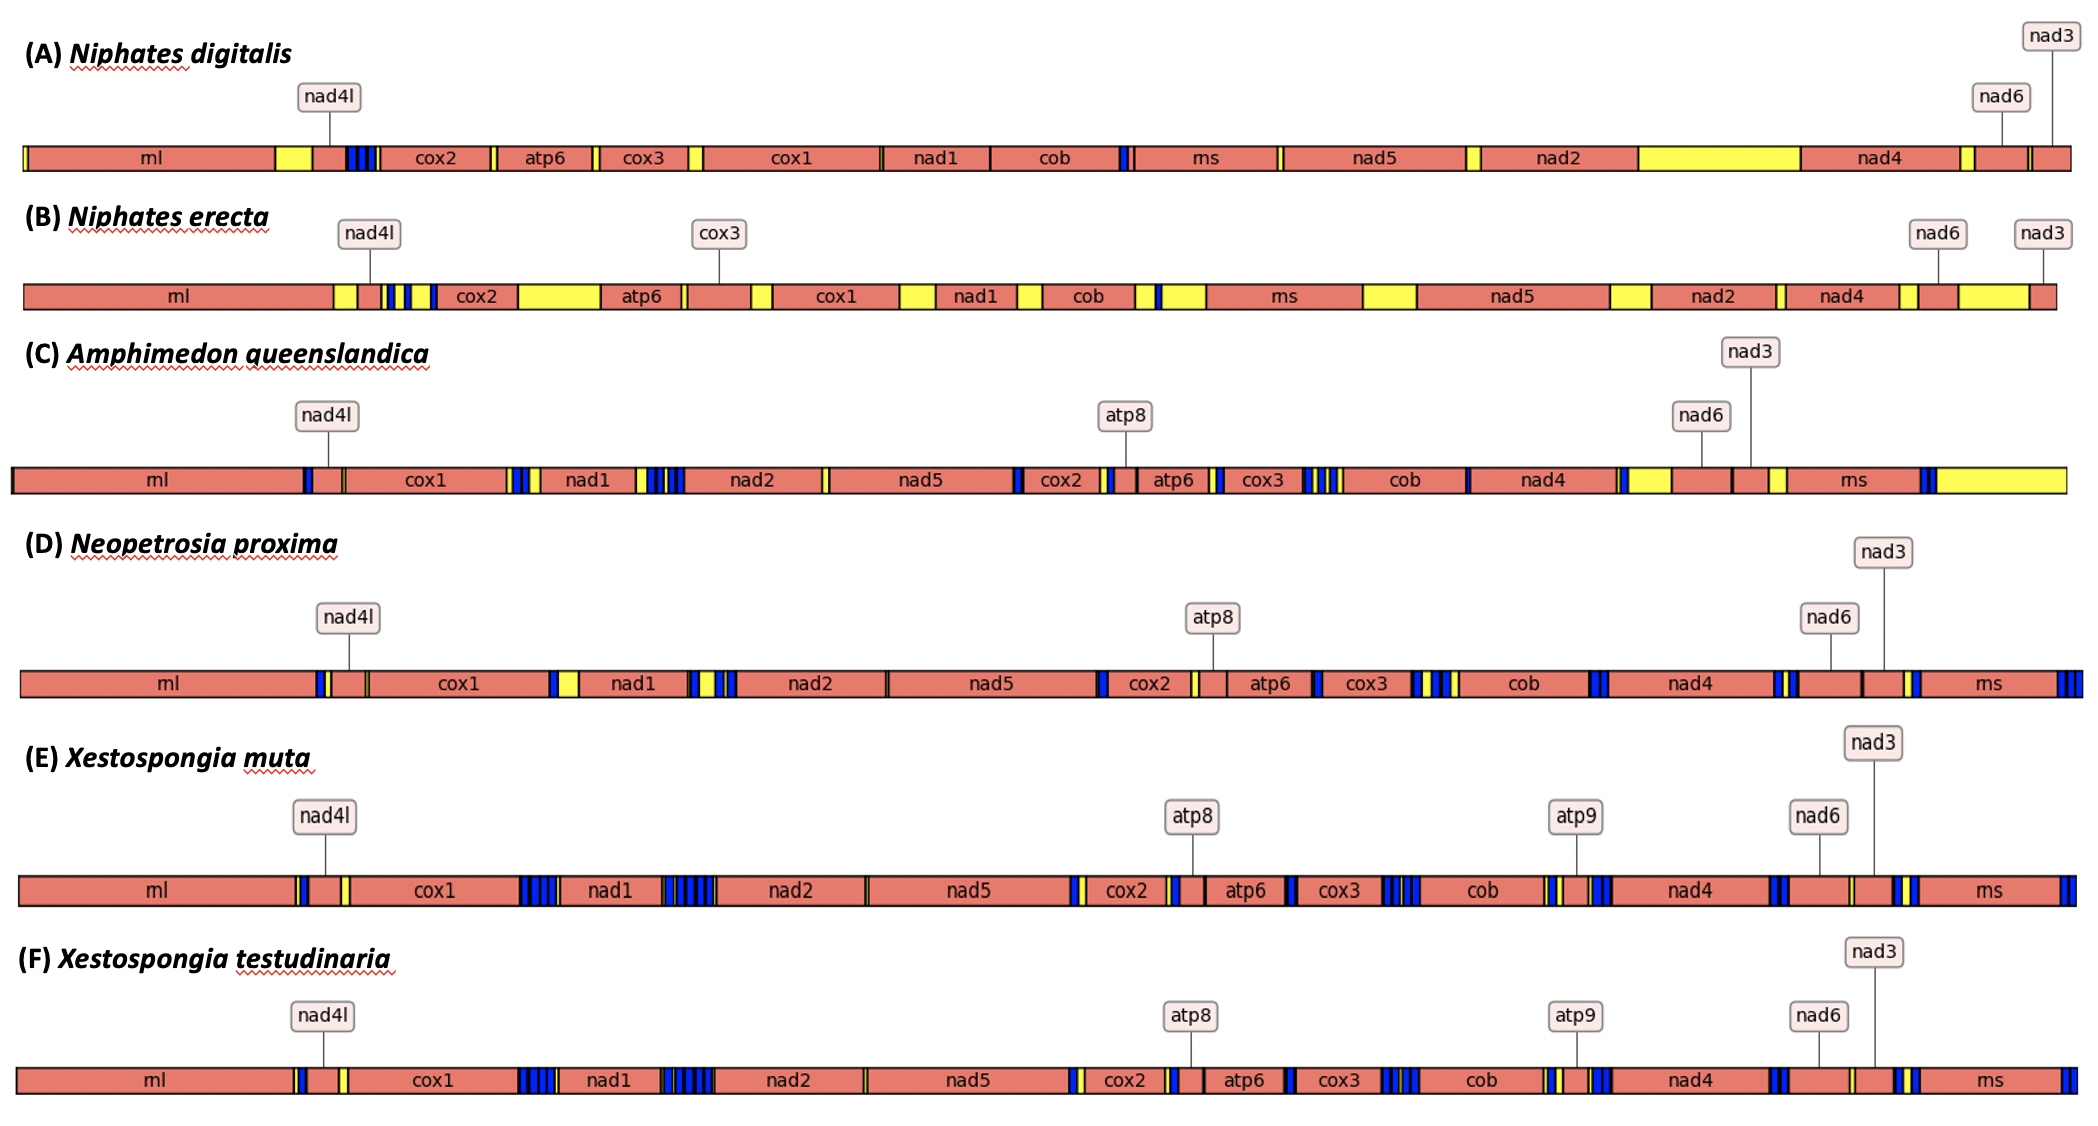
\includegraphics[width=1.0\textwidth]{Figures/figure 1.png}
    \caption{(A) The mitochondrial genome of \emph{Niphates erecta}. (B) The mitochondrial genome of \emph{Niphates digitalis}. Red are coding genes, yellow is intergenic regions, blue is tRNA genes, purple is insertions, and green are step-loop elements.}
\end{figure}

\subsection{Gene Loss}
Interestingly, both \emph{Niphates digitalis} and \emph{N. erecta} are missing the genes for \emph{atp8} and \emph{atp9}, which code for subunits of mitochondrial ATP synthase.  

Transcripts of \emph{atp8} and \emph{atp9} were found in the transcriptome of \emph{Niphates erecta}, suggesting a move to the nuclear genome. An analysis of the \emph{atp9} nucleotide sequences from \emph{Niphates erecta} and \emph{Amphimedon queenslandica} as compared to \emph{atp9} sequences in other species showed... An analysis of the \emph{atp8} sequence from \emph{Niphates digitalis}'s transcriptome showed... [Still needs to be done]

\subsection{Gene Order}
While the gene order for both species was the same, (see Figure 1), the gene order was strikingly different than other demosponge mitochondrial genomes previously reported. 

To better understand the differences, gene orders from 62 mitochondrial genomes from G3 and G4 demosponges were compared to the gene orders of \emph{Niphates digitalis} and \emph{Niphates erecta}. [NEED TO DO ANOTHER ANALYSIS FOR THIS] Generally, the mitochondrial genes formed clusters of genes in a specific order that were almost always found together. The order of the clusters change, but little variation to the cluster identities were seen in the other demosponge gene orders. Clusters are presented in Figure 2.

\begin{figure}[htp]
    \centering
    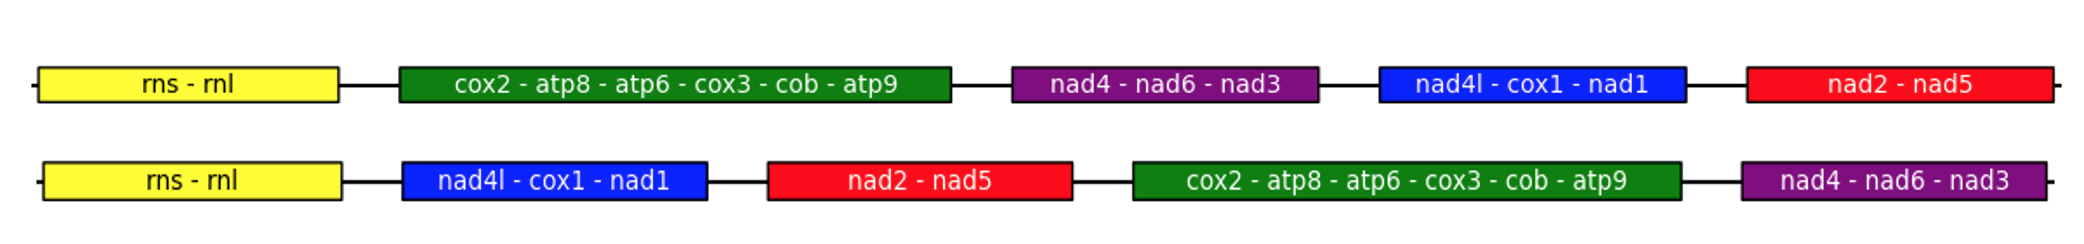
\includegraphics[width=1.0\textwidth]{Figures/figure 2.png}
    \caption{The two different configurations of gene orders seen in G3 and G4 sponges. In the 62 species studied, little variation was seen in this pattern until \emph{Niphates digitalis} and \emph{Niphates erecta}.}
\end{figure}

The five clusters alternate in pattern, with no cluster of NADH genes situated next to each other. As seen in Figure 2, G3 sponges show a pattern of the \emph{rnl} group, \emph{cox1} group, \emph{nad2} group, the \emph{cox2} group, and the \emph{nad4} group. Individual genes are typically separated by tRNA genes, but the identity of tRNA genes between genes is not consistent. 

The mitochondrial genomes for both \emph{Niphates} species do not match either pattern identified in G3 or G4, despite being most closely related to the G3 sponge \emph{Amphimedon queenslandica}. Multiple clusters have been rearranged, and the cluster orders seen in G3 and G4 are not seen in \emph{Niphates}. The gene order for both species is seen in Figure 2b. To begin, \emph{rnl} and \emph {rns} are not found together, and instead are found with 8 and 6 genes on either side of them. The gene \emph{nad4l} has been separated from the \emph{cox1} group and is instead found by the \emph{cox2} group. The \emph{cox2} group appears to have undergone serious rearrangement, as evidenced by the \emph{cox1} group appearing between \emph{cox3} and \emph{cob}. In addition, the \emph{nad2} group has been flipped, with \emph{nad5} appearing before \emph{nad2}. Finally, breaking the pattern of the NADH gene groups not appearing side-by-side, the \emph{nad4} group is found next to the flipped \emph{nad2} group. 

\subsection{Multiple insertions found in the \emph{N. erecta} mt-genome}
The primary difference between the two genomes lies in the novel insertions identified in the \emph{N. erecta} mt-genome. When compared to \emph{N. digitalis, N. erecta} has a multitude of insertions present. Eighty insertions have been identified, ranging in size from a few base pairs to large sections up to 650 bps long, and have a similar nucleotide composition to the genome as whole. The majority of insertions fall into intergenic regions, but are also found in serveral genes:\emph{cox2, atp6, nad1, nad5, rnl}, and \emph{rns}, of which \emph{cox2, atp6, nad1,} and \emph{nad5} are protein-coding.

As a few of these insertions fall into protein-coding genes, it was important to understand the impact these insertions are having on down-stream products. The majority of insertions were in-frame, but two of these genes - \emph{atp6} and \emph{nad5} - have out-of-frame insertions. The distribution of in-frame and out-of-frame insertions are seen in Table 1. **INSERT TRANSCRIPTOME ANALYSIS HERE WHEN COMPLETED**

\begin{center}
\begin{tabular}{ |c|c|c|c| } 
 \hline
 \textbf{Gene}& \textbf{Number of Inserts} & \textbf{In-Frame} & \textbf{Out-of-Frame}\\
 \hline
 \emph{cox2}  & 4  & 4 & 0 \\
\hline
\emph{atp6} & 5 & 4 & 1 \\
\hline
\emph{nad1} & 2 & 2 & 0 \\
\hline
\emph{nad2} & 1 & 1 & 0 \\
\hline
\emph{nad5} & 4 & 1 & 3 \\
\hline
\end{tabular}

\caption{\textbf{Table 1:} Summary of insertions in \emph{Niphates erecta}. The total number of insertions are reported in column 2, the number of in-frame insertions in column 3, and the number of out-of-frame insertions in column 4.}
\end{center}

Regardless of the impact these insertions and deletions have on proteins and downstream functions, they do account for the discrepancy in genomes size between species. The \emph{N. digitalis} and \emph{N. erecta} genomes are 25525 bps and 18285 bps, respectively. The majority of this length difference can be attributed to the increased number of intergenic regions and insertions seen in \emph{N. digitalis}. Intergenic regions account for 24.2\% of \emph{N. digitalis}'s genome, as opposed to 13.77\% in \emph{N. erecta}, and insertions in protein-coding areas account for an additional [INSERT PERCENTAGE HERE] of \emph{N. digitalis}'s mitochondrial genome.

However, the two genomes show an identical nucleotide composition.  The \emph{N. digitalis} genome has a GC and AT content of XX and YY, while \emph{N. erecta} has a GC and AT content of YY and YY. Without the insertions being considered, \emph{N. digitalis} has a GC and AT content of XX and YY respectively.  

\subsection{Inverted Repeats}

Further analysis of \emph{N. digitalis}'s insertions and intergenic regions found that many contain inverted repeat sequences. The locations of these can be seen in Figure Y. Inverted repeats have previously been identified in other sponge species, and their function is unknown. These inverted repeats were isolated from the genome, and like the insertions, analyzed with NCBI BLAST. They returned no close sequence relations under any parameters. Alignments of the \emph{Niphates} inverted repeats showed that majority of repeats have the same general sequence, see Figure Z, and when folded form hairpin-like structures.

The inverted repeats fall into four different motifs, the structures of which can be seen in Figure Z. [IF YOU HAVE SUGGESTIONS ABOUT HOW TO SHOW THESE LET ME KNOW] The majority of inverted repeats contain motif 1. Motif 1 contains a highly conserved 11-nucleotide stem with a 4 nucleotide loop. Before and after the stem-loop is not conserved. Motif 2 shows a similar pattern, though it is less common. It contains a well-conserved 12 nucleotide stem with a 3 nucleotide loop at the top. In addition, bases before the stem-loop are typically conserved. Motif 3 is another large, well conserved stem-loop, with a 13 base stem and a six nucleotide loop. As with the others, the regions on either side of the stem are not conserved. Motif 4 is much smaller, with a 5 nucleotide stem and a 6 nucleotide loop. 

Many of the inverted repeats appear and stem-loop elements appear in a large sections together, results in dense regions of stem-loop elements. The function of these stem-loop elements is unknown. In addition, the same motifs appear at different points across the genome, and do not group together in particular locations.

\subsection{tRNA content and sythetases}
One of the novel traits seen in some sponge mitochondrial genomes is a lack of mitochondrial tRNAs. \emph{Niphates digitalis} and \emph{Niphates erecta} are no exceptions. Both genomes had the same four mitochondrial tRNAs - Y, I, M, and W. These tRNAs fall into the same place in the genome, with Y, I, and M between \emph{nad4l} and \emph{cox2}, and W being between \emph{cob} and \emph{rns}. As compared to other demosponges genomes, the location of these tRNAs tend to change, and don't maintain a stable position across species.

Alignment of these tRNA genes with mt-tRNA genes from other demosponge species shows these tRNAs to be closely related to the same tRNA gene in other species, with no abnormal structures. This indicates there has been no gene recruitment to cope with the loss of mitochondrial tRNAs, and why these particular tRNA genes were retained is unknown.

\end{document}